% !TEX TS-program = xelatex

% This is the LaTeX template
% for "Constructions", a very simple
% modification of the standard 
% LaTeX article class. The 
% main.tex file of this template
% as well as localstuff.tex
% can be used without attribution
% under the public domain CC-0 license.
% The bibliography style unified.bst
% is used under the LaTeX Project 
% Public License v1.3c.

% Note that the file has to be compiled
% in XeLaTeX! If you work in Overleaf,
% XeLaTeX should already be selected 
% (you can check this by taking a look at
% Menu > Compiler). Some LaTeX editors
% will also recognize the correct
% compiler automatically because of
% the "magic command" at the beginning
% of this script.

% to keep the present file readable,
% packages & commands have been relocated
% to localstuff.tex:
\documentclass[12pt,a4paper,twoside]{article}

%%%%%%%%%%%%
% PACKAGES %
%%%%%%%%%%%%

\usepackage[T1]{fontenc}
\usepackage{tabularx, colortbl}
% \usepackage[english]{babel}
\usepackage[margin=3cm]{geometry}
% \usepackage{newtxtext,newtxmath}
\usepackage{xcolor}
\definecolor{ochre}{RGB}{204, 119, 34}
\usepackage[colorlinks=true,linkcolor=black,citecolor=black,filecolor=magenta,urlcolor=ochre]{hyperref}

\usepackage[final,nopatch=footnote]{microtype}

\usepackage{
	enumitem,
	multicol,
	multirow,
	linguex,
	amssymb,
	microtype,
	stmaryrd,
	natbib,
	amsmath,
	booktabs,
	calculator,
	verbatim,
	titling,
	fontspec,
	changepage,
	float,
    multirow
}

% Paper license
\usepackage[
    type={CC},
    modifier={by},
    version={4.0},
]{doclicense}

% set bibliography style
\bibliographystyle{unified}
\setcitestyle{aysep={},notesep={: }}

% heading font:
\newfontfamily\headingfont[]{IBM Plex Sans}

% main font:
\usepackage{CharisSIL}

% packages:
\usepackage[]{titlesec}
\usepackage[hang]{footmisc}
\usepackage[nocenter]{qtree}
\usepackage[normalem]{ulem}
\usepackage{graphicx}
\usepackage{fancyhdr}



\setlength{\bibsep}{0.0pt}


\setlength{\intextsep}{4pt plus 2pt minus 2pt}
%\setlength{\parindent}{0em}
\setlength{\parskip}{2pt}
\setlength{\parindent}{1em}
\renewcommand{\firstrefdash}{}
\linespread{1}

\newcommand{\ii}{\={i}}
\newcommand{\red}[1]{\textcolor{red}{#1}}
\newcommand{\Reference}{\\ \textcolor{white}{.}\hfill}

% header style for all but first page
\pagestyle{fancy}
\fancyhf{}
\renewcommand{\headrulewidth}{0pt}

% header style for first page
\fancypagestyle{plain}{%
  \fancyhf{}% clear all header and footer fields
  \renewcommand{\footrulewidth}{0.4pt}
  \lfoot{\sffamily \footnotesize \textbf{Corresponding author(s):} \correspondingauthor}
  \rfoot{\thepage}%
}


% set head height
\setlength{\headheight}{14.49998pt}

\titleformat*{\section}{\large\bfseries\headingfont}
\titleformat*{\subsection}{\normalsize\bfseries\headingfont}
\titlespacing*{\section}{0em}{15pt}{10pt}

% get the volume number:
\SUBTRACT{\the\year}{2008}{\volume}

% for vertical centering text in tabularx X column
\renewcommand\tabularxcolumn[1]{m{#1}}

% column types for tabularx
\newcolumntype{L}{>{\raggedright\arraybackslash}X}
\newcolumntype{R}{>{\raggedleft\arraybackslash}X}
\newcolumntype{C}{>{\centering\arraybackslash}X}

\usepackage{caption}
\captionsetup{font=footnotesize}


% no vertical space in lists
\setlist{nosep}

% remove vertical space after verbatim environment
\usepackage{etoolbox}
\makeatletter
\preto{\@verbatim}{\topsep=0pt \partopsep=0pt }
\makeatother

% enumitem package seems to override this
% behavior, so we also add
% (thanks to https://tex.stackexchange.com/questions/43331/control-vertical-space-before-and-after-verbatim-environment)
\AtBeginEnvironment{verbatim}{\setlist[trivlist]{nolistsep}}

% for citations in genitive
\newcommand{\citegen}[1]{\citeauthor{#1}'s (\citeyear{#1})}


% For the **running head**, please enter a 
% short title of the paper as well as 
% the name/s of the author/s here (for
% papers with more than 2 authors,
% use First Author et al.). The full
% title and the full list of authors and
% affiliations is to be entered below (see
% "Insert title and author/s").

\fancyhead[LO]{Author 1 \& Author 2}
\fancyhead[RE]{Short title}
\fancyhead[RO, LE]{\thepage}

% Please enter the corresponding author(s) here:
\newcommand{\correspondingauthor}[1]{Random Author, University of Somewhere, random.author@uni-somewhere.edu}


% if you want to customize the
% hyphenation of individual words,
% you can do so here. This can be
% particularly helpful if you get
% the notorious "overfull hbox"
% error.

\hyphenation{
    hy-phe-na-tion
    num-bered
}


\raggedbottom
\begin{document}


% make sure that first page doesn't
% have running heads:
\thispagestyle{plain}

% first page header:
% DOI and Creative Commons license
\newcolumntype{Y}{>{\raggedleft\arraybackslash}X}

\noindent
\begin{tabularx}{\textwidth}{XY}
\multirow{2}{*}{\doclicenseImage[imagewidth=0.5\linewidth]} & \small{\textit{Constructions} \volume \  (\the\year)} \\
& \small{doi{10.24338/cons-xxx}} \\
\end{tabularx}

\vspace{30pt}
\begin{center}
    \LARGE\headingfont{\textbf{Redes de monitoreo de basura espacial}}
\end{center}

\begin{center}
\vspace{4pt}
\large
    Abundis-Patiño Jesus, Kokina Tatiana \& Mendoza-Araiza Daniel\textsuperscript{1}
    
\small
   \textsuperscript{1} Centro de Astronomía, Universidad Autónoma de Sinaloa

\end{center}


% Abstract section
\begin{small}
\begin{center}
\vspace{9pt}
\textbf{Resumen}    
\end{center}

\begin{adjustwidth}{20pt}{20pt}
\small \noindent En este artículo se hace una discusión sobre los diversos centros que realizan actividades de monitoreo de basura tecnológica espacial; sus tareas, algunos de sus logros y su organización. Al mismo tiempo se presenta un breve recuento histórico sobre el desarrollo de la problemática de la basura espacial y el surgimiento de un ente internacional que pone en marcha estos centros con el objeto de realizar observaciones, evaluar riesgos para la humanidad y establecer reglamentos para las misiones espaciales.
\end{adjustwidth}


\end{small}





% Initial section
\vspace{10pt}
\section*{Introducción}\label{Sec:Introduction}

La basura tecnológica espacial ha tomado un interés público que se ha visto reflejado tanto en la comunidad científica como por los medios de comunicación tradicional. El aumento en el interés a este problema es resultado de un incremento masivo en los viajes espaciales relacionados principalmente con la colocación de satélites para distintas aplicaciones; satélites de comunicación, climatológicos, de investigación del espacio, entre muchos otros. Mientras la puesta en marcha de estos proyectos asiste múltiples necesidades de la sociedad, tales como la comunicación en locaciones remotas, los equipos utilizados en estos también introducen desafíos importantes al terminar su operación, entre los cuales tenemos el daño a nuevos objetos puestos en órbita e incluso el riesgo para los seres humanos durante su caída a la Tierra.

Dada la relevancia que ha tomado la cantidad de restos no funcionales en el espacio en la actualidad, la ONU ha tomado la iniciativa de atender esta situación mediante la creación de una división especializada en el tema.



\section{Linguistic examples} \label{sec:linguex}

For linguistic examples, we use the ``linguex" package. The package is relatively easy to use, see the manual for examples: \url{https://ftp.rrze.uni-erlangen.de/ctan/macros/latex/contrib/linguex/doc/linguex-doc.pdf}. Just insert \verb!\ex.! to start an example, and use \verb!\\! for line breaks. You can refer to examples like example \ref{ex:myExample} below by adding labels to the individual examples using the \verb!\label{...}! command and referring to the label you chose via \verb!\ref{the_label}!. In this way, you can also refer to sub-examples like \ref{ex:myExamplea} and \ref{ex:myExampleb}.
 
\ex. \label{ex:myExample}
 \ag. \textit{Das} \textit{ist} \textit{ein} \textit{Beispiel}. \\
  This is an example. \\
  `This is an example.' \label{ex:myExamplea}
  \bg. \textit{Ein} \textit{Beispiel} \textit{ist} \textit{das}. \\
  an example is this \\
  `This is an example.' \label{ex:myExampleb}


\section{Figures}

Inserting figures is easy, while it can be a bit harder to place them where you would like to see them. The \href{https://www.overleaf.com/learn/latex/Inserting_Images}{Overleaf tutorial} provides a good starter. Usually you can just work with the code in this template. Please make sure that you have high-resolution figures (at least 300 dpi). Like the linguistic examples discussed above, you can label figures and then refer to them using \verb!\ref{the_label}! or, if you want to add the word ``Figure" (or ``Table", in the case of tables) automatically, \verb!\autoref{the_label}!.


\begin{figure}[H]
    \centering
    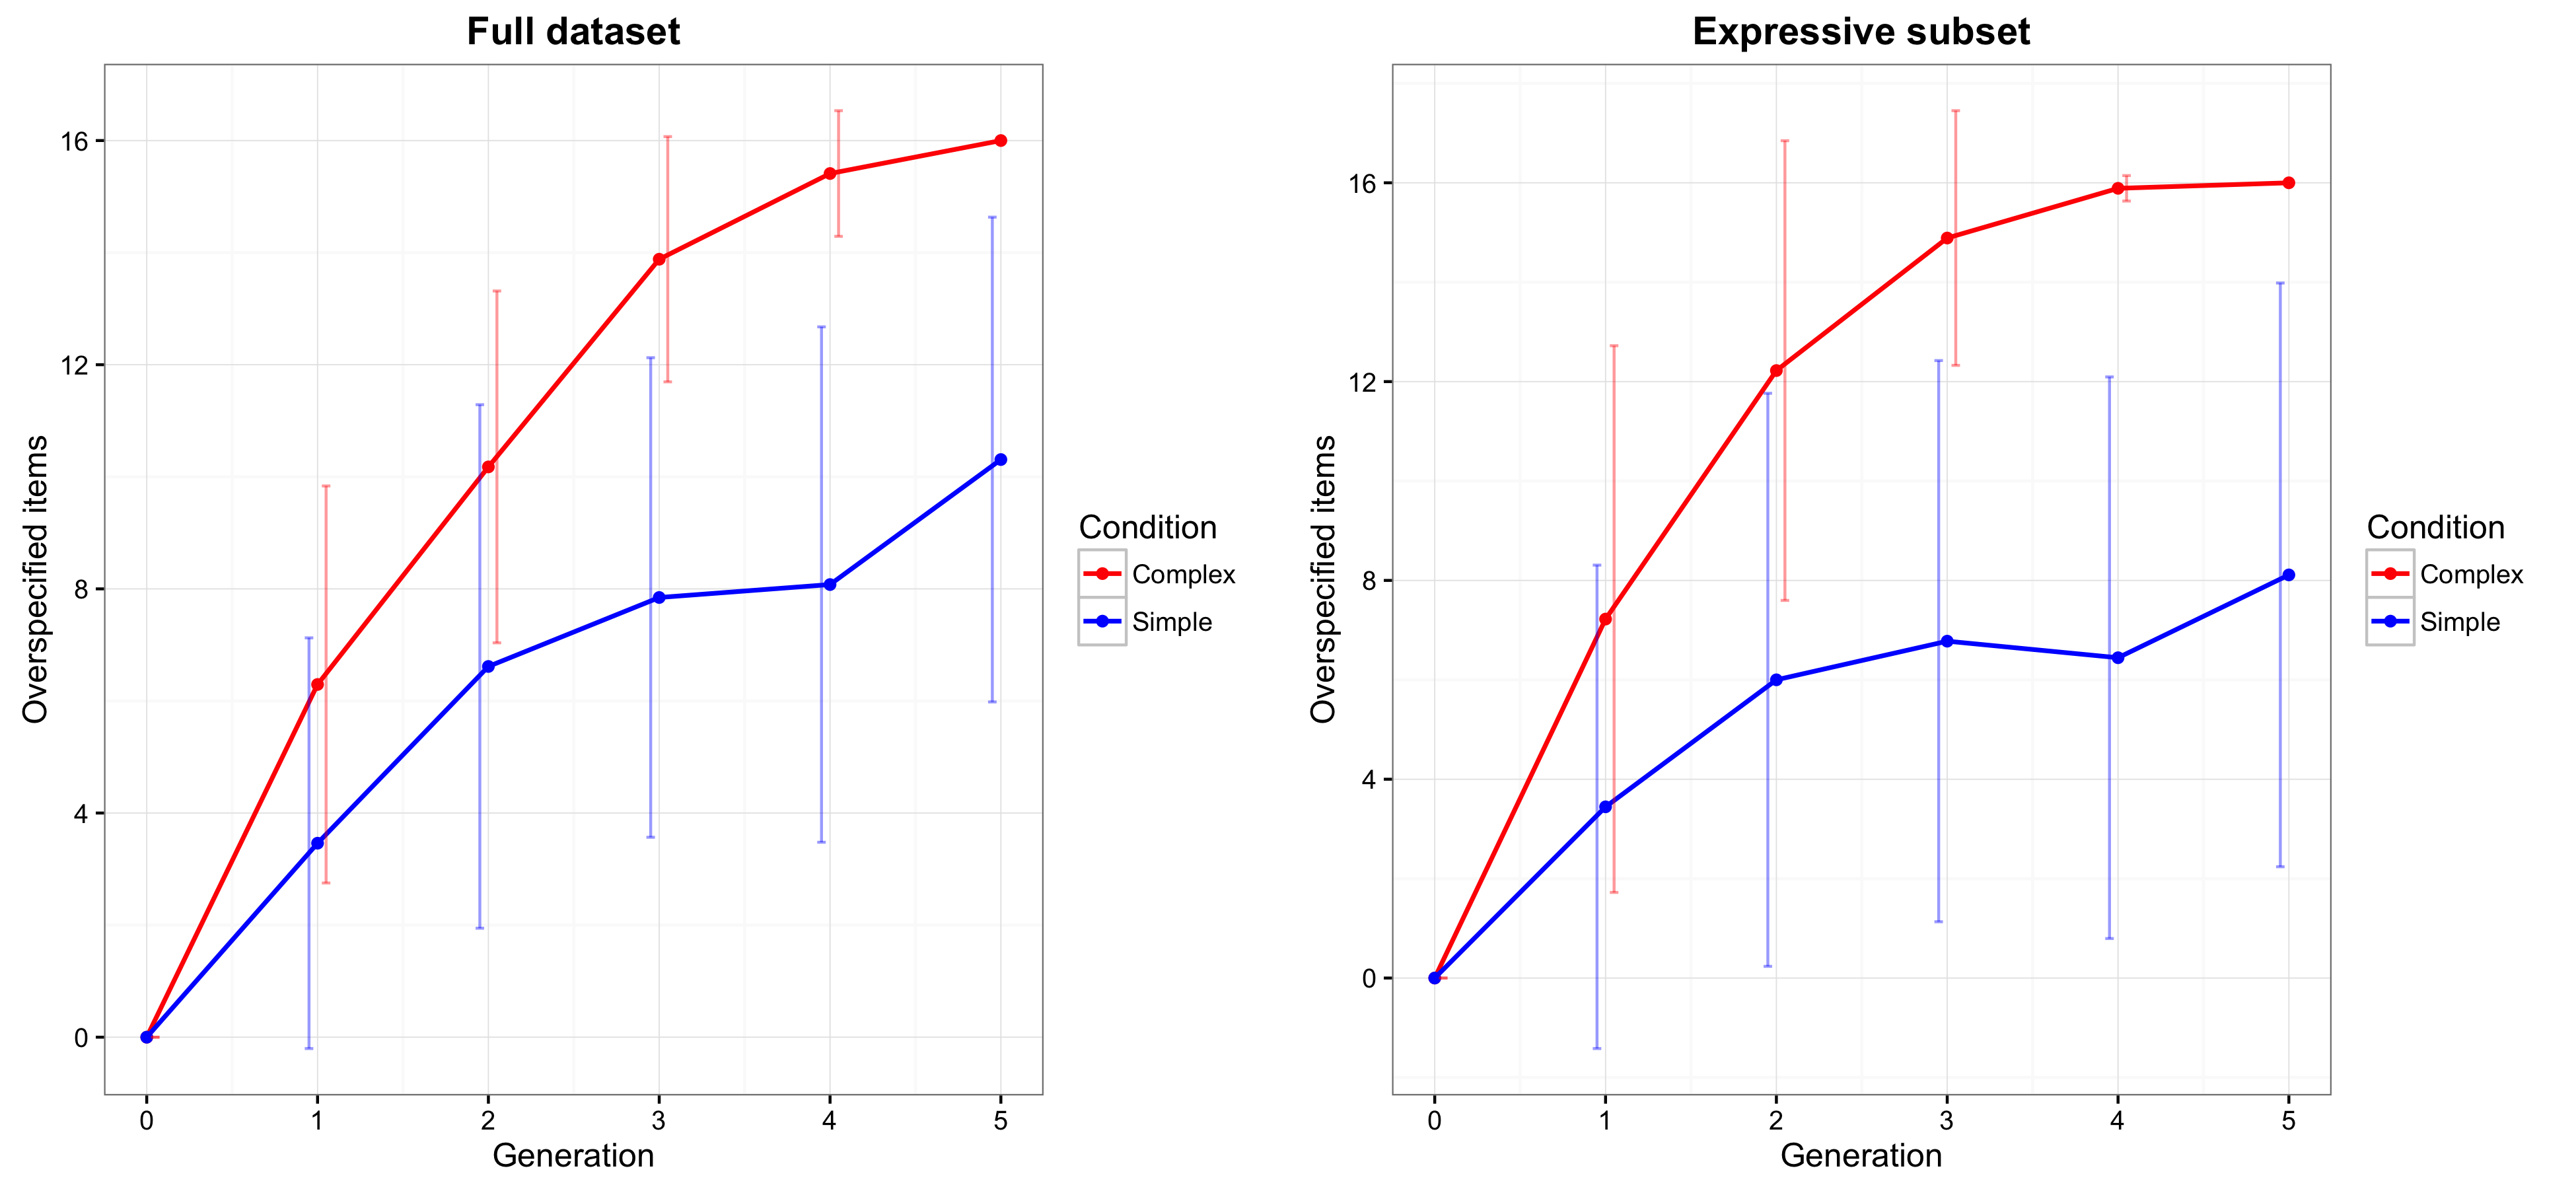
\includegraphics[width=\textwidth]{Figures/Figure2.png}
    \caption{A sample figure}
    \label{fig:my_first_figure}
\end{figure}

\noindent The \href{https://ftp.tu-chemnitz.de/pub/tex/macros/latex/contrib/float/float.pdf}{float package} can be used to customize the position of figures and tables. For example, \autoref{fig:my_first_figure} and \autoref{fig:my_second_figure} are forced to appear at a specific position in the text using the \verb![H]! command. If there is no reason to position a figure or table at a specific point in the text, you can also use a less strict configuration and let \LaTeX \  choose the position automatically. If you use \verb![H]! and start a new paragraph afterwards, please make sure to start the paragraph with the command \verb!\noindent! to avoid indentation.

\begin{figure}[H]
    \centering
    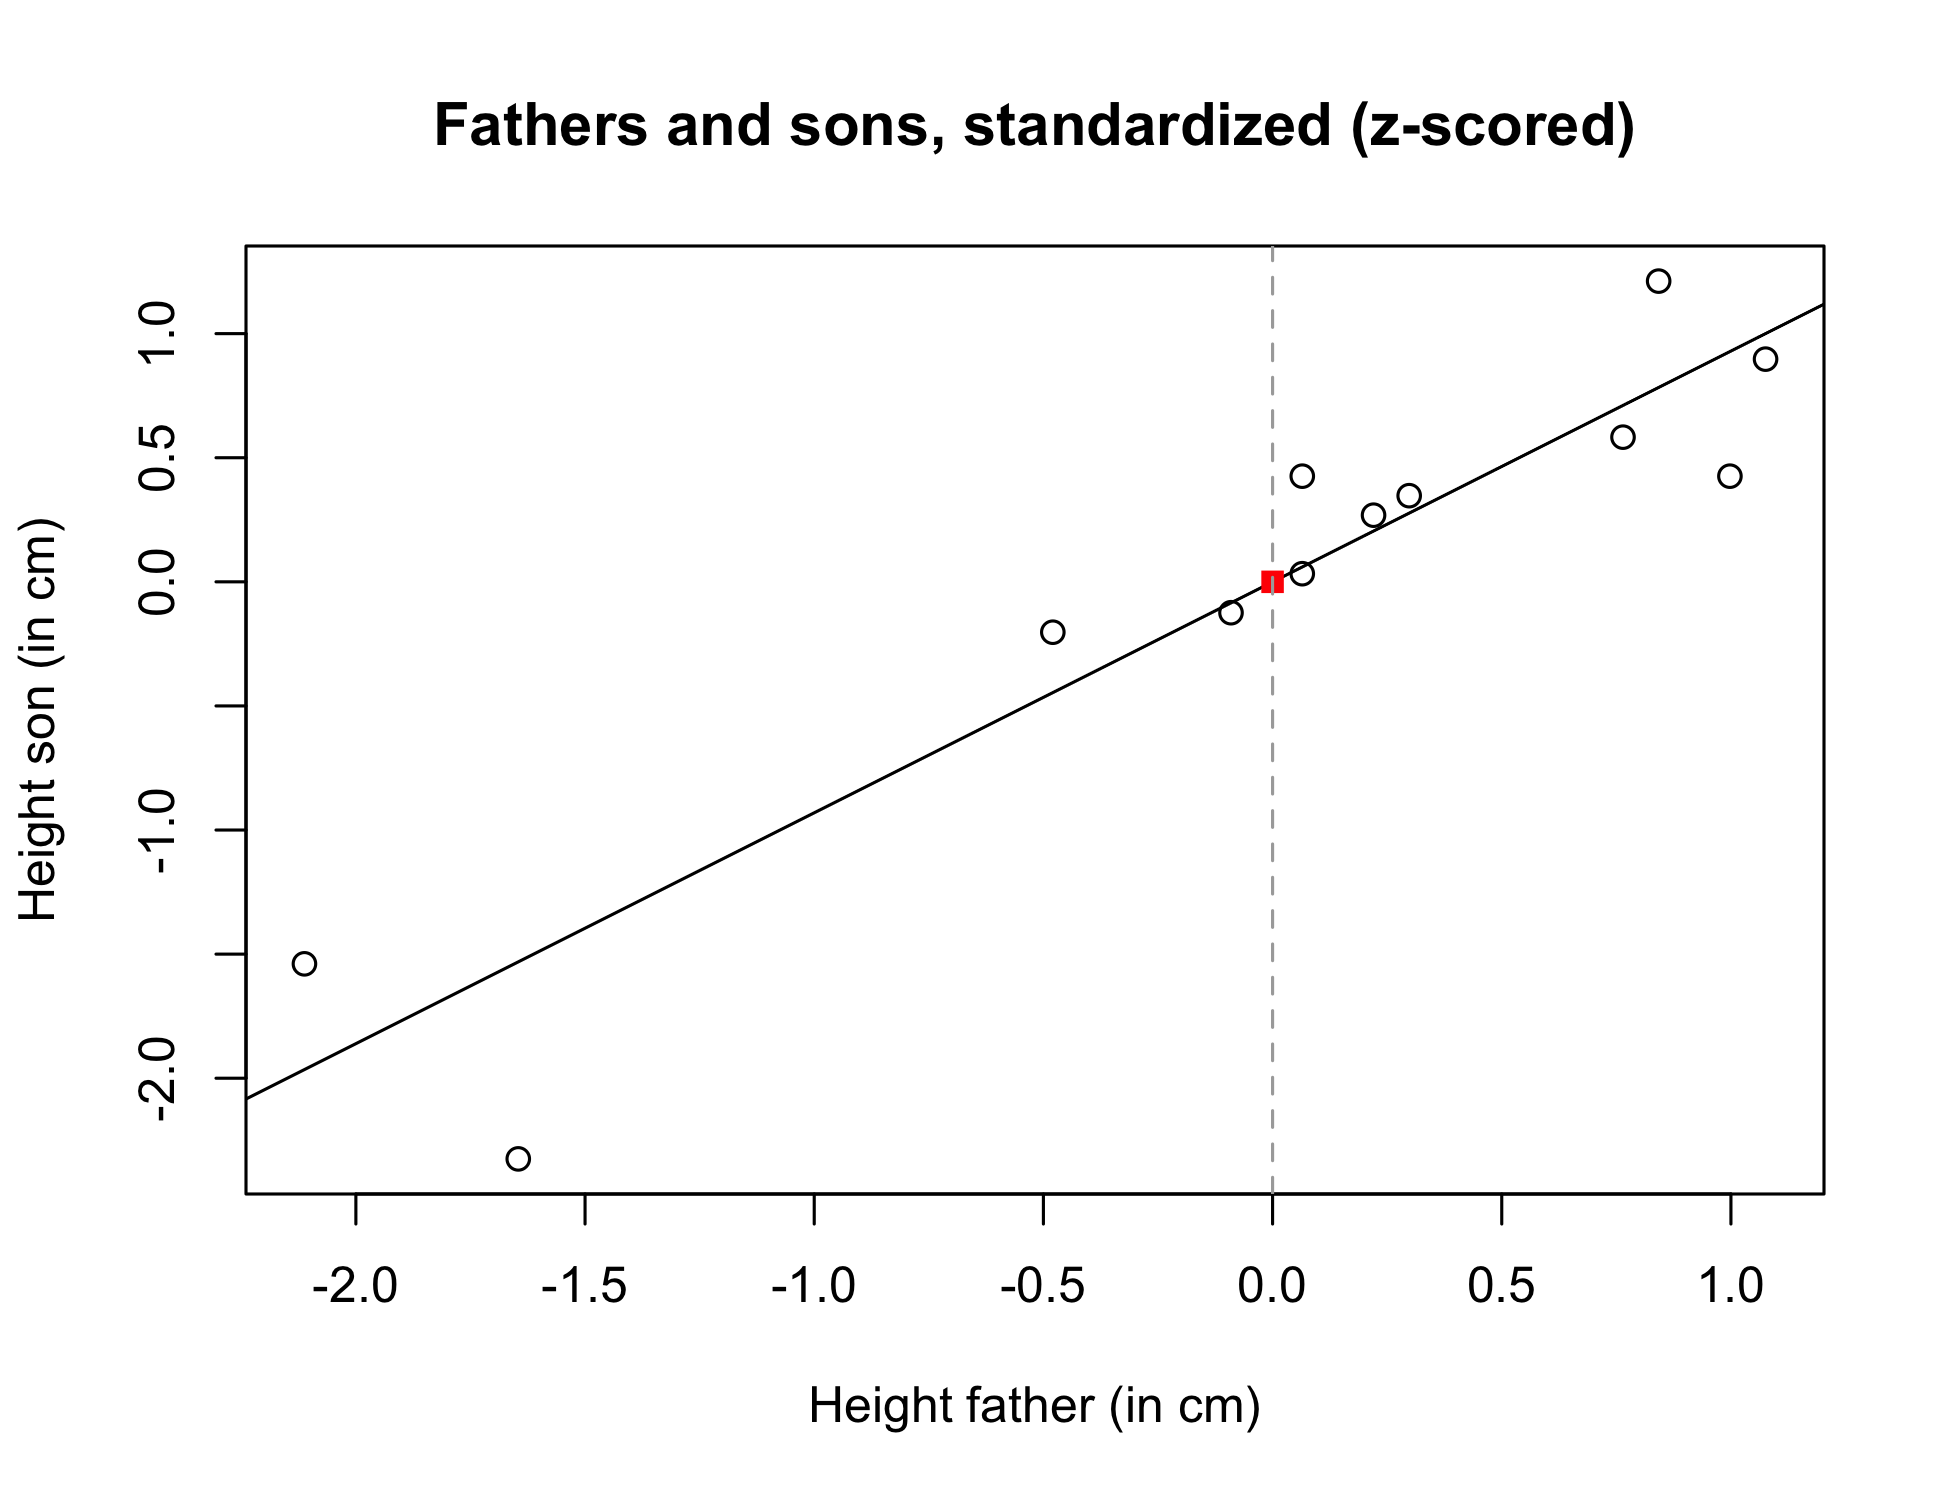
\includegraphics[width=0.8\textwidth]{Figures/fathersandsons4.png}
    \caption{Another sample figure}
    \label{fig:my_second_figure}
\end{figure}

\subsection*{Reusing figures} \label{sec:reusing}

If you reuse figures from published work, including your own, please make sure that you are allowed to do so. In most cases, you will need to obtain written permission from the copyright holder (usually the publisher) to re-use figures, unless the original paper has been published under an open license such as CC-BY. We generally recommend to double-check if re-using the figure is actually necessary. If it is, please make sure to obtain written permission for re-using the figure. When re-using figures that cannot be published under a creative commons license, please add a short statement to the license information at the bottom of the paper, e.g. ``Figure x from Author (Year: page), re-used by permission from Calisota University Press, is excluded from this license."


\section{Tables}

Adding tables is, admittedly, one of the more challenging aspects of \LaTeX \ typesetting. Luckily, there are a few resources that help you generate tables, such as \url{https://www.tablesgenerator.com/}. 

\begin{table}[H]
    \sffamily \begin{tabularx}{\textwidth}{ | L | L | }
    \hline
         bla & blubb  \\
         \hline
         blah & blub \\
         \hline
    \end{tabularx}
    \caption{A very simple table}
    \label{tab:my_first_table}
\end{table}

\noindent We recommend to use the \href{https://ctan.org/search?phrase=tabularx}{tabularx} package, which is a bit more complicated to use than the normal ``tabular" environment, but it gives you more flexibility in customizing the tables, and makes it easier to print it in text width. In the localstuff.tex file, we have defined the column types L (left-aligned), C (centered), and R (right-aligned) so you don't have to use the full commands that tabularx usually requires. In the simplest case, therefore, constructing a table is as easy as in the source code of \autoref{tab:my_first_table}. For more elaborate tables in which some rows and columns are merged, check the source code of \autoref{tab:my_complicated_table}.


\begin{table}[H]
    
    \begin{tabularx}{1\textwidth}{| L | L |R |}
    \hline
         \rowcolor[gray]{.9} Col1 & Col2 & Col3 \\
        \hline
        blubb &  blibb & 2 \\
        \hline
        \multicolumn{2}{|>{\hsize=\dimexpr2\hsize+2\tabcolsep+1\arrayrulewidth\raggedright\relax}X |}{ Lorem ipsum dolor sit amet, } & bla\\\hline
        \rowcolor[gray]{.8} \multicolumn{3}{|>{\hsize=\dimexpr3\hsize+4\tabcolsep+2\arrayrulewidth\centering\relax}X |}{ Lorem ipsum dolor sit amet, }\\
        \hline
        
bla & blabb & 22 \\
\hline
    \end{tabularx}
    \caption{A more compilcated table}
    \label{tab:my_complicated_table}
\end{table}

\normalfont

\section{Special characters}

From 2025 onwards, \textit{Constructions} uses the open font \href{https://software.sil.org/charis/}{Charis SIL} by default, which supports a broad array of Unicode characters. With the \verb!\symbol{...}! command, you can easily add more Unicode characters using a font of your choice, e.g. \verb!{\fontspec{Symbola}\symbol{"1F5A4}}! will be displayed as {\fontspec{Symbola}\symbol{"1F5A4}}. 

\section{Citations and references}

``Constructions" follows the \href{https://www.linguisticsociety.org/resource/unified-style-sheet}{Unified Style Sheet for Linguistics Journals}. Working with \LaTeX \  and BibTeX, you don't have to do the formatting manually, though. All references you cite should be in the bibliography.bib file in BibTeX format. We strongly recommend using a reference manager like \href{https://www.zotero.org/}{Zotero}. Zotero allows you to copy and paste entries in BibTeX format, thus making it much easier to work with \LaTeX. 

For inserting citations, use \LaTeX's citation syntax:

\begin{itemize}
    \item Use \verb!\citep{...}! for inserting citations in parantheses, e.g. \citep{Example2}.
    \item Use \verb!\citet{...}! to insert citations in the format Author/s (Year), as in \citet{Example2}.
    \item Use \verb!\citeauthor{...}! and \verb!\citeyear{...}! if you just want to cite the author or the year, without parantheses. This can be helpful if you cite something within parantheses (as in this example, see \citeauthor{Example1} \citeyear{Example1}).
    \item If you want to use a possessive 's in references, you can use the custom command \verb!\citegen{...}! defined in the localstuff.tex file, as in: \citegen{Example1} definition of constructions.
\end{itemize}

\subsection*{Troubleshooting}

If there are problems with the bibliography, this can have several reasons:

\begin{itemize}
    \item Some Zotero plugins (like Better BibTeX) change the ``Year" field in the BibTeX entry to ``Date". In this case, you'll have to change all instances of ``Date" to ``Year" in the bibliography file.
    \item If you want to keep sentence-internal capitals in the citations (e.g. when quoting German titles, such as \citeauthor{Example3} \citeyear{Example3}), make sure that the relevant words are enclosed in curly brackets. If you export the BibTeX entries from Zotero, you usually won't have to worry because it does so automatically.
\end{itemize}

\section*{Obligatory declarations}

To meet the requirements of pertinent publication ethics standards, we kindly ask you to add the following declarations at the end of your paper:

\begin{itemize}
    \item \textbf{Conflict of interest statement:} Typically, there will be no conflict of interest to state. If this is the case, just write something like ``The author/s has/have no competing interests to declare."
    \item \textbf{Data availability statement:} If you have analyzed data, please add a link to a public repository in line with our \href{https://constructions.journals.hhu.de/about}{Open Data Policy}. 
    \item \textbf{Ethics statement:} If you work with sensitive data (including, but not limited to, experiments involving underage participants or data from clinical populations), please add an ethics statement. 

    
\end{itemize}

\section*{Conflict of interest statement}

The authors declare none. % change if necessary

\section*{Data availability statement}

The data and analysis scripts for the present paper are available at [[ADD LINK]].

\section*{Ethics statement}
\textit{(Delete if not applicable)}

\noindent The present study was reviewed and approved by [[Full name and affiliation of ethics committee, date and/or reference number of ethics vote]]. All participants provided their written informed consent to participate in this study.

\section*{License}
\doclicenseIcon \doclicenseText

\noindent \textit{Constructions} uses the CC-BY (``By Attribution") license by default, i.e. everyone can copy, share, and build upon your paper, given that they give proper attribution. If you prefer a more restrictive license, you can change it in the localstuff.tex file, e.g. to
\begin{itemize}
    \item CC-BY-SA (``Share alike"), i.e. any derivative work has to use the same or a compatible license;
    \item CC-BY-SA-ND (``No derivatives"), i.e. the work has to be shared under the same or a compatible license, and derivative works such as translations are excluded.
\end{itemize}

\noindent See the \href{https://creativecommons.org/}{Creative Commons website} for more information about the different licenses.

If necessary, please add statements about elements that are exluded from the CC license as described in Section \ref{sec:reusing}.

\bibliography{bibliography}

\end{document}
